\documentclass[pdf,slideColor,nocolorBG,accumulate,total,gyom]{prosper}
\usepackage[italian]{babel}
\usepackage[utf8]{inputenc}
\usepackage{graphicx}
\usepackage[T1]{fontenc}
\usepackage{hyperref}

\author{Emanuele Santoro}
\email{manu@salug.it}
\date{31 Dicembre 2008}
\title{Il sistema operativo GNU/Linux}
\institution{ITIS E. Fermi - Lecce}


%--------------- LOGO DEFINITION ------------
\Logo{
\includegraphics[width=1cm,height=1.28cm]{immagini/hackergotchi.eps}\small{\emph{\blue{http://santoro.tk}}}}
%---------------- END LOGO DEFINITION --------

\begin{document}

\maketitle

\begin{slide}{Presentazione}
	\center{Il Sistema operativo GNU/Linux}

Il sistema operativo GNU/Linux è un sistema operativo di tipo UNIX (la
definizione esatta è \emph{UNIX-like}, vedremo in seguito che significa)
caratterizzato principalmente dalla sua licenza: la GNU GPL
(\emph{General Public License}).

\end{slide}

\overlays{4}{
\begin{slide}{Com'è questo Linux?}
\onlySlide*{1} {
{\tiny
{\black
GNU/Linux può essere visto in molte forme diverse. Quasi tutte seguono
delle linee di principio simili, ma in genere ognuna ha una
particolarità, ognuna è stata creata per fare qualcosa di particolare.

Possiamo dire, ognuna ha un obiettivo ben precisa.

Sebbene il sistema operativo Windows, purtroppo enormemente più diffuso
di GNU/Linux, abbia {\bfseries un} solo modo di gestire il desktop,
GNU/Linux da all'utente la possibilità di gestire autonomamente, e di
{\bfseries decidere} come gestire il proprio desktop.

Ci sono ambienti come KDE o Gnome che tendono ad essere completi ed a
gestire ogni aspetto dell'uso del computer: dal movimento del mouse allo
scaricamento della posta, passando per la gestione dei files e delle
cartelle, delle connessioni di rete e delle risorse del computer.

Ci sono ambienti invece dove tutto il resto viene lasciato all'utente,
che può farlo a mano oppure predisporre altri programmi per farlo.
Questi ambienti hanno lo svantaggio, di essere più difficili da usare 
e più lunghi da imparare ad usare. Danno però una possibilità di 
personalizzazione quasi totale.

Queste slides sono state create sotto uno di questi: 
\href{http://www.nongnu.org/ratpoison/}{Ratpoison}.
}
}
}


\onlySlide*{2} {
Questo ad esempio è KDE, versione 3.5.10

\flushright{
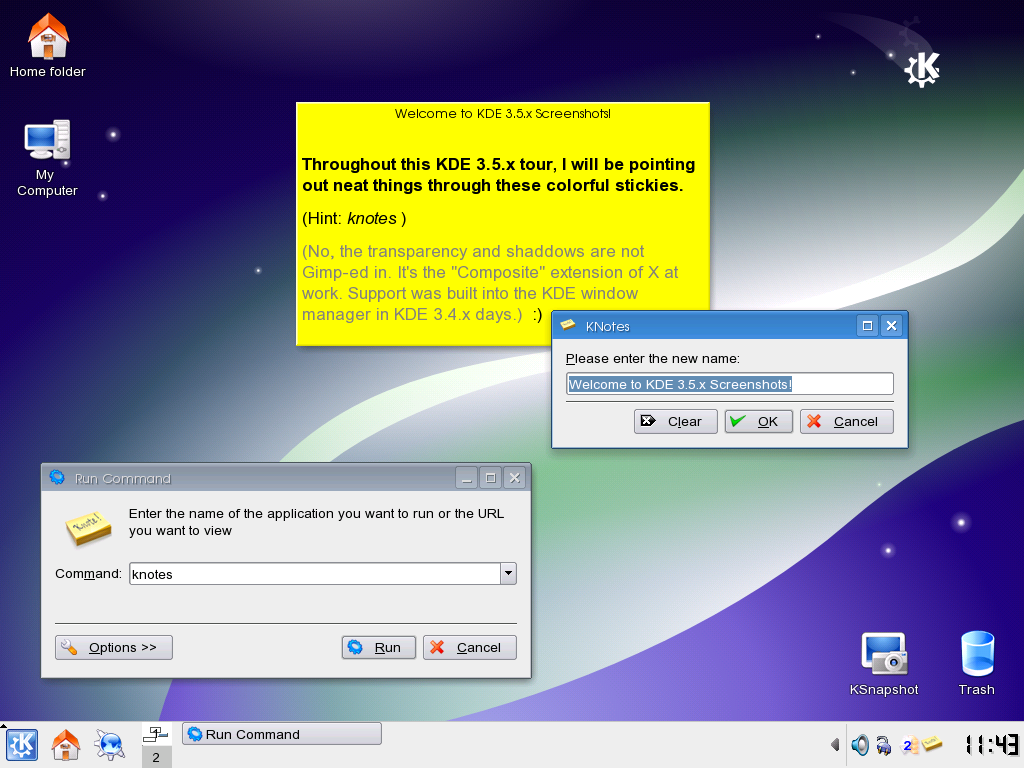
\includegraphics[width=8cm,height=6cm]{immagini/kde.eps}
}
}


\onlySlide*{3} {
Gnome 2.24:

\flushright{
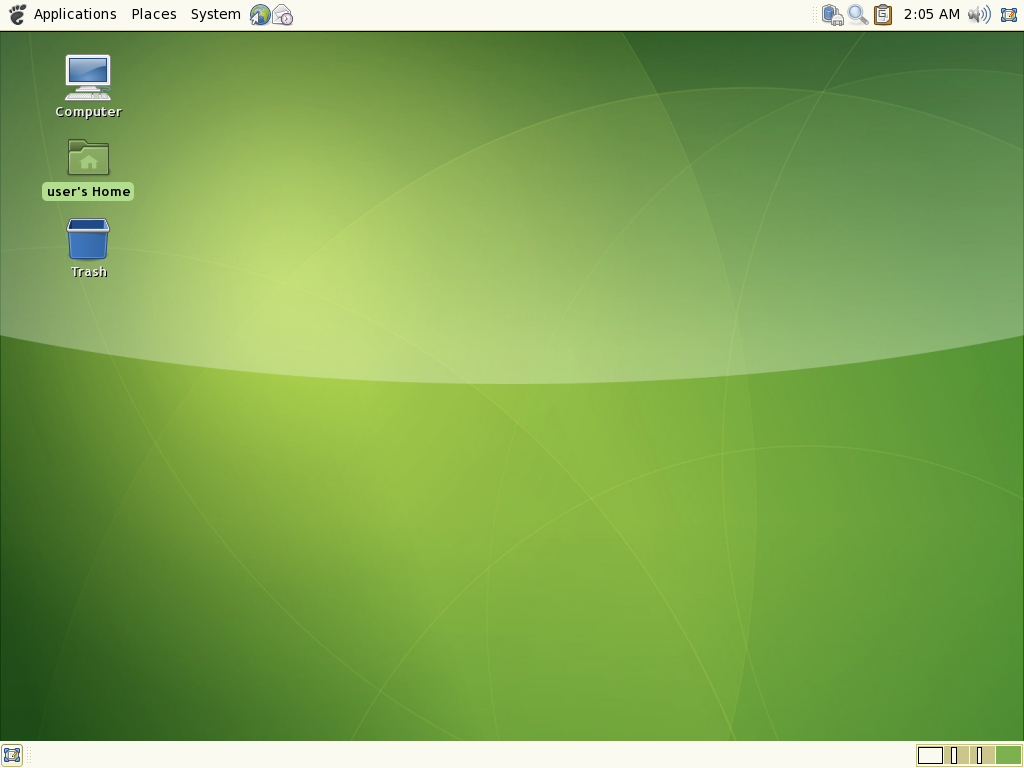
\includegraphics[width=8cm,height=6cm]{immagini/gnome.eps}
}
}


\onlySlide*{4} {
Questo invece è Ratpoison.
\flushright{
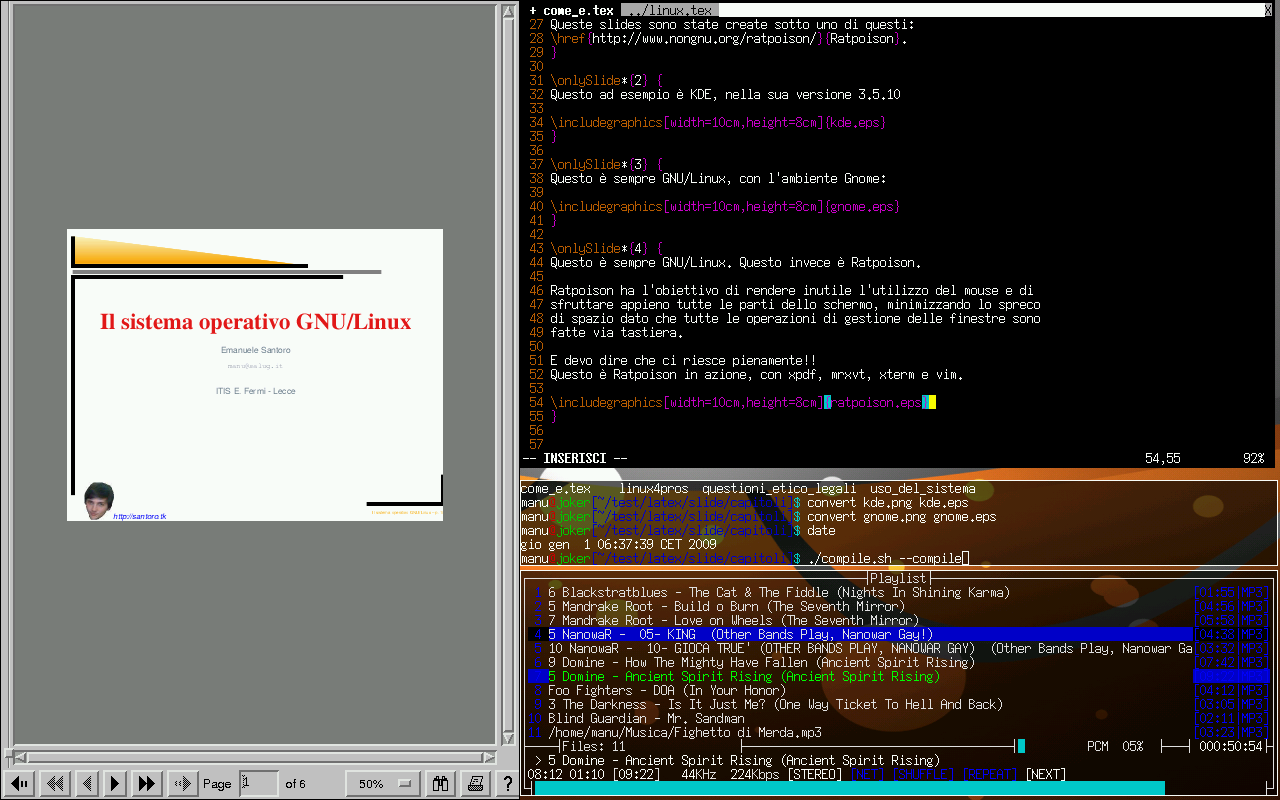
\includegraphics[width=10cm,height=6cm]{immagini/ratpoison.eps}
}
}



\end{slide}}


\begin{slide}{Questioni etico-legali}
Ogni software ha una licenza.

La licenza definisce cosa è permesso fare e cosa non è permesso fare con
un software.

Inoltre, ogni software ha una sua storia dietro.

Vediamo le particolarità della licenza di GNU/Linux e le sue storie.

\end{slide}


\overlays{2} {
\begin{slide}{GNU/Linux... Ma che vuol dire?}

\onlySlide*{1} {
In queste pagine si parla di GNU/Linux... Ma non si chiamava "Linux" e
basta?
La risposta e no, ma anche si.
Linux, per essere precisi, indica il kernel, il \emph{cuore} del sistema
operativo... Quel pezzo di codice che sta a diretto contatto con il
ferro, ecco.

GNU, invece, è tutto il resto.

I programmi che usi, i driver, le interfacce grafiche, il browser,
l'editor... Quello è GNU.
}

\onlySlide*{2} {
\begin{itemize}
	\item[-] GNU sfrutta Linux per girare (dei programmi devono
	essere eseguiti da un kernel... se non c'è il kernel, dove
	girano i programmi?)
	\item[-] Linux sfrutta GNU per avere qualcosa da far girare (il
	kernel serve a far girare i programmi... se non ci sono
	programmi, a che server il kernel?)
\end{itemize}

{\huge GNU + Linux = GNU/Linux }
}

\end{slide} }


\overlays{3}{
\begin{slide}{GNU: Gnu's Not Unix}

{\red {\small Si è parlato spesso di GNU\dots Cos'è il "Progetto GNU" ?}}

\onlySlide*{1}{
Bisogna sapere che in origine il mondo dell'informatica era molto
diverso. Quando i computer occupavano ancora intere stanze, tutto il
software circolava liberamente con il solo scopo di progredire nella
tecnologia e nell'informatica. UNIX era il sistema operativo in voga
all'epoca. Nato per fini più pratici che teorici, era distribuito
liberamente.
}

\onlySlide*{2}{
\tiny{
Un giorno, molte aziende cominciarono ad acquistare UNIX,
modificarlo e cambiare la sua licenza così chè esso divenne chiuso, a
pagamento e chi lo usava non poteva avere accesso al suo codice
sorgente, non poteva studiarne il funzionamento, modificarlo qualora ne
avesse bisogno e gli stessi sviluppatori che lo avevano creato non potevano, legati da
contratto, rivelare niente che riguardasse il sistema operativo.

La forte comunità scientifica che si era creata intorno ad UNIX, fatta
di scambio libero del sapere, codice libero, licenze praticamente
assenti, aiuto reciproco e amicizia venne di colpo stroncata.
}}

\onlySlide*{3}{
{\tiny
Un ricercatore, però, si oppose a tutto questo.

Rifiutando contratti favolosi, posti di lavoro eccellenti e paghe
profumate, Richard Matthew Stallman decise che avrebbe creato un suo
sistema operativo.

Un sistema operativo che avrebbe avuto l'obbiettivo principale di essere
\emph{libero}. 

Un sistema operativo che fosse simile ad UNIX, visto che UNIX funzionava
abbastanza bene, ma che non ne fosse una copia pari pari. Così venne GNU: 
}

\center{Gnu's Not Unix}

\begin{tabular}{lcr}

\includegraphics[width=0.25\columnwidth,height=0.30\textheight]{immagini/gnu.eps} &%
&%
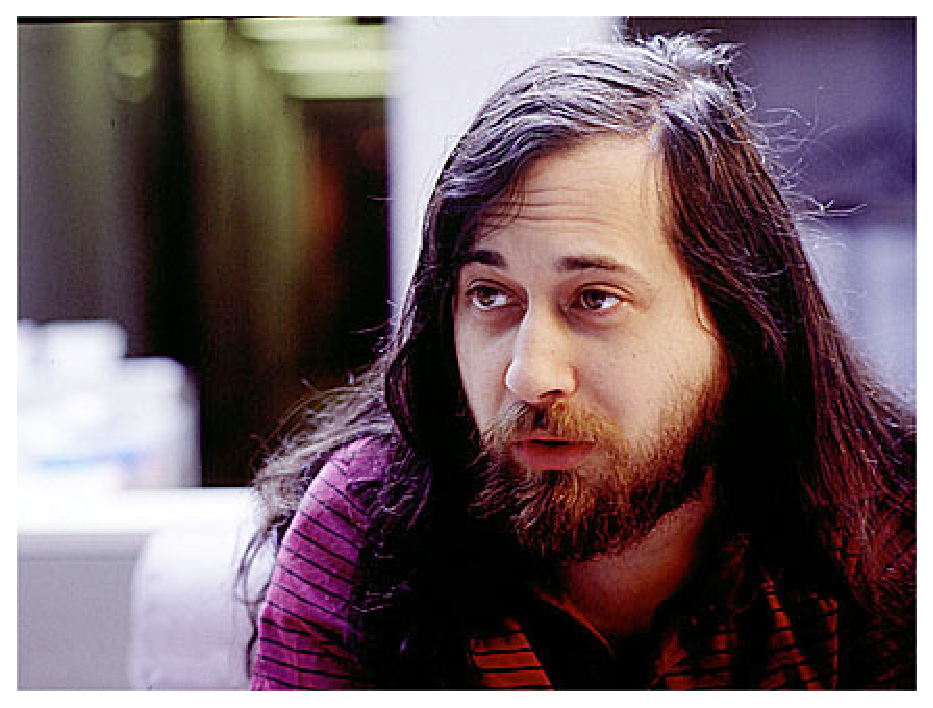
\includegraphics[width=0.25\columnwidth,height=0.30\textheight]{immagini/stallman.eps}%

\end{tabular}



}

\end{slide}}


\begin{slide}{Il Software Libero}

{\small 

{\red Che vuol dire Software Libero?} 

Questo termine viene dall'inglese "Free Software", e si riferisce al
software sia free in senso di libero che free nel senso di gratuito.

In inglese infatti, "\emph{free}" vuol dire sia \emph{libero} che
\emph{gratuito}.

Il software è libero perchè rispetta le quattro libertà fondamentali
dell'utente, ed è gratuito perchè non è richiesta alcuna somma per
l'utilizzo del software.

Questo tuttavia non esclude la possibilità di guadagnare con il Software
Libero, anzi.
}

\end{slide}


\overlays{5}{
\begin{slide}{{\small Le quattro libertà fondamentali}}
Quali sono le quattro libertà fondamentali?



\begin{itemize}

\fromSlide*{2}{\item[-] Libertà  di eseguire il programma, per
qualsiasi scopo e senza nessuna limitazione}

\fromSlide*{3}{\item[-] Libertà di studiare il programma e modificarlo}

\fromSlide*{4}{\item[-] Libertà di copiare il software in modo da
aiutare il software }

\fromSlide*{5}{\item[-] Libertà di migliorare il software e di
distribuirne liberamente i miglioramenti, in modo tale che tutta la
comunità possa trarne beneficio }

\end{itemize}

\end{slide}}


\begin{slide}{La GPL: General Public License}
{\small 
Essendo GNU/Linux un sistema operativo vero e proprio, ampiamente
utilizzato e diffuso, ha bisogno di una licenza vera e propria, che
abbia vero valore legale. 

La \emph{\href{http://www.fsf.org/}{Free Software Foundation}}, ente
creato da Stallman per supportare il Progetto GNU, ha redatto negli anni
una Licenza vera e propria, in lingua \emph{legalese}, adatta a
preservare il software e mantenerne la libertà.

Questa licenza e la General Public License.

Ci sono state diverse versioni della GPL, e la più recente è la terza 
versione, pubblicata il 29 Giugno 2007.

}
\end{slide}


\overlays{4}{
\begin{slide}{Linux}
{\small
Spendiamo ora qualche parola riguardo a Linux:

\onlySlide*{1}{
{\black
Linux era il progetto \emph{personale} di Linus Torvalds, allora
studente all'università di Helsinki (Finlandia), che stava cercando un
sistema operativo abbastanza economico da usare sul cuo computer di
casa, un 386.

Torvalds inizia così lo sviluppo e poi rilascia pubblicamente il suo
lavoro sotto la licenza GPL. Piano piano qualcuno comincia ad usare
Linux. Lo usa, trova dei problemi, e li segnala, o li risolve e spedisce
a Torvalds il suo contributo.

Con il tempo sempre più persone usano Linux, il kernel cresce.
}
}

\onlySlide*{2}{
{\black
Linux e GNU non erano in origine progetti correlati.

Intorno al 1991, GNU era quasi completato ma gli mancava un kernel, e
partì lo sviluppo di Hurd, un microkernel che al giorno d'oggi non è
ancora completamente sviluppato.

Intanto, Torvalds continua a sviluppare il suo kernel.

Qualcuno non collegato nè a Torvalds, nè a GNU, prova a vedere cosa si
ottiene mescolando GNU, a cui manca un kernel, a Linux, a cui manca
tutto il resto.
}
}

\fromSlide*{3}{
{\black
Nasce GNU/Linux... Ed il resto ormai è storia! \emph{;-)}
}
}

\fromSlide*{4}{
\flushright{
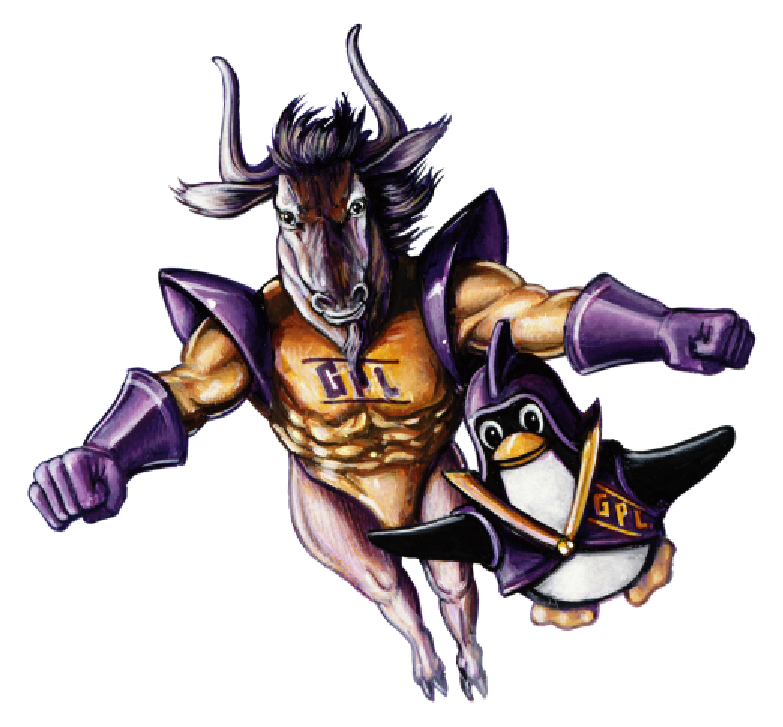
\includegraphics[width=6cm,height=6cm]{immagini/dynamicduo.eps}
}
}

}
\end{slide} }


\begin{slide}{Questioni tecniche}
Andiamo ora a vedere come è strutturato il sistema operativo GNU/Linux,
evidenziandone i punti di forza.
\end{slide}


\begin{slide}{Gli strati del kernel}

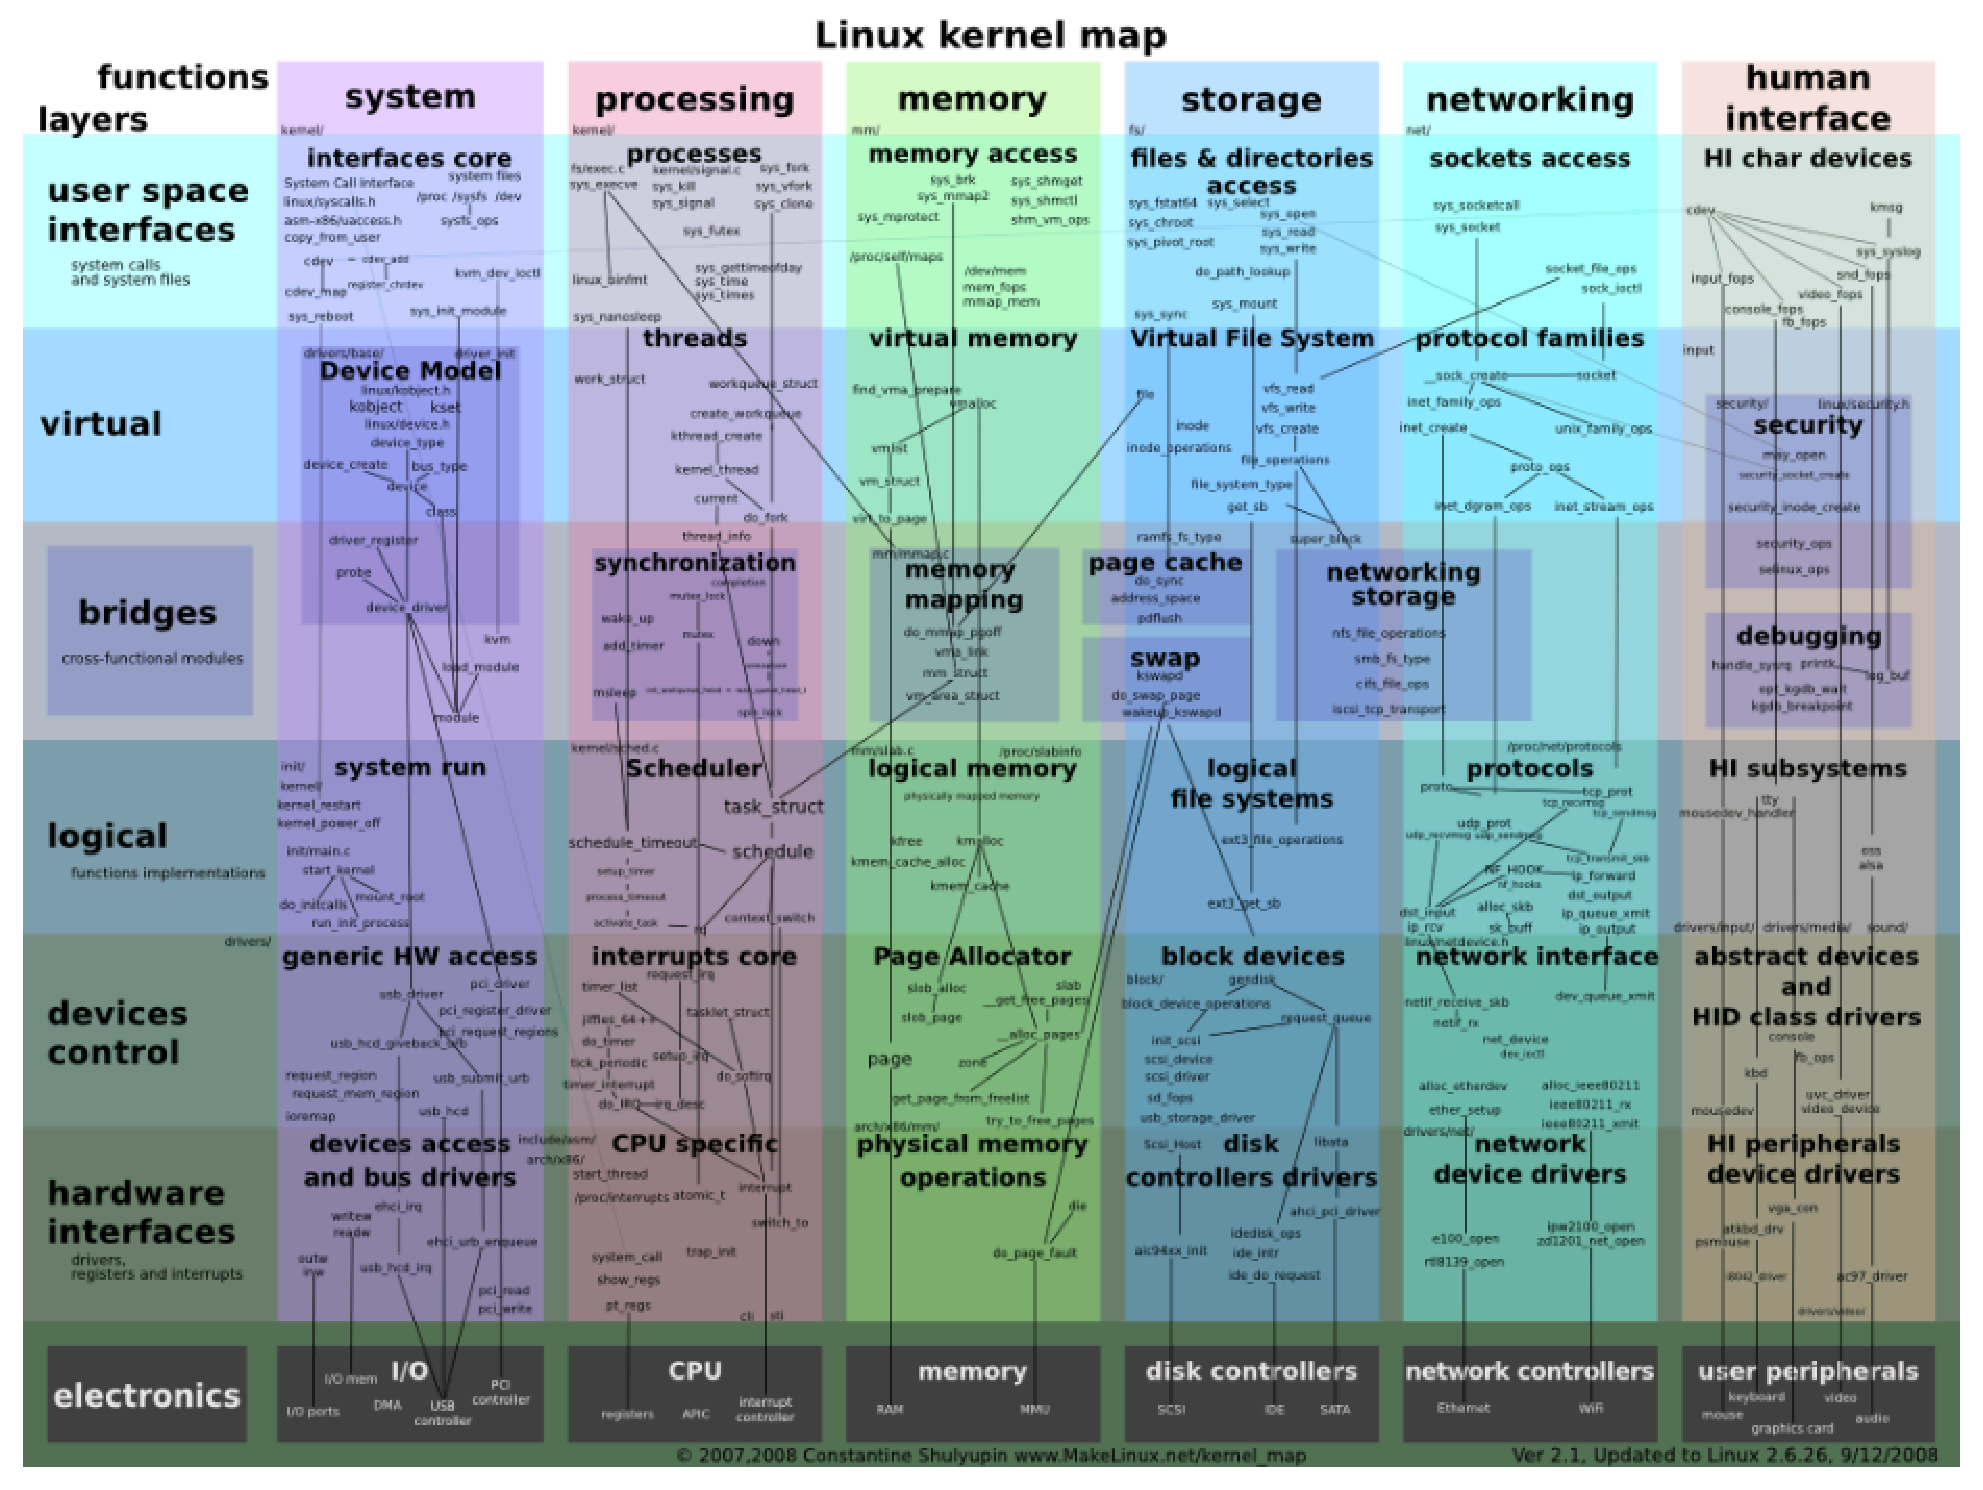
\includegraphics[width=0.80\columnwidth,height=0.80\textheight]{immagini/linux_map.eps}

\flushright{
{\small Questo è lo schema interno del Kernel Linux\dots}}

\end{slide}


\overlays{5}{
\begin{slide}{Layout del sistema operativo}
A differenza di Windows, GNU/Linux non è un sistema operativo "tutto in
uno":

\begin{itemize}
	\onlySlide*{2}{\item[-]I programmi sono parte separata dal sistema}
	\onlySlide*{3}{\item[-]L'interfaccia grafica è parte separata del sistema }
	\onlySlide*{4}{\item[-]Il filesystem non è parte del sistema operativo}
\end{itemize}


\onlySlide*{5}{
\flushright{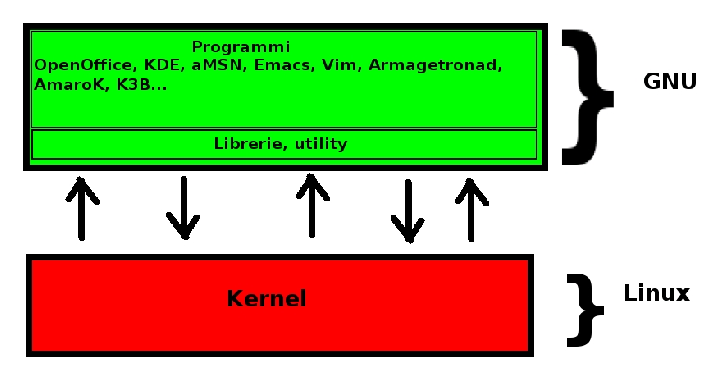
\includegraphics[width=8cm,height=6cm]{immagini/linux_layout.eps}}
}

\end{slide}
}


\overlays{2}{

\begin{slide}{L'interfaccia grafica}
{\small
GNU/Linux ha una potentissima modalità grafica che si basa su un
componente chiave: \emph{Xorg}.

\onlySlide*{1}{
La più importante caratteristica di Xorg è che è \emph{network-based}.
Che vuol dire? Vuol dire che tutte le operazioni vengono svolte via
rete.

Xorg si compone di un server e di tanti client.
}

\onlySlide*{2}{
	\flushright{ 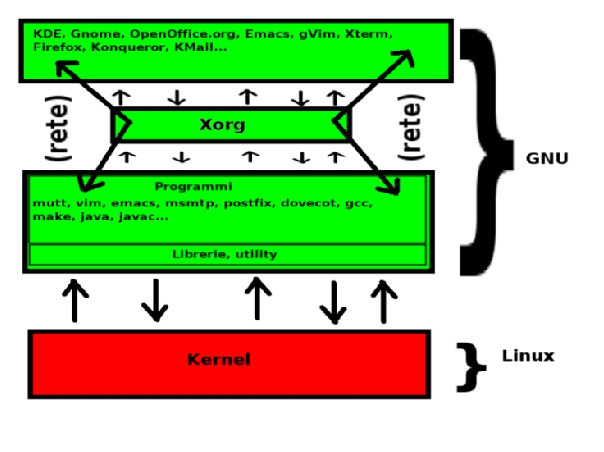
\includegraphics[width=8cm,height=6cm]{immagini/xorg_layout.eps} }
}

}

\end{slide}}



\begin{slide}{La gestione del sistema}
{\small
\flushleft{
La gestione del sistema in linux è abbastanza diretta e semplice, anche
se può sembrare apparentemente difficile.

In linea generale, tutti programmi hanno diversi modi di funzionare,
e questi modi vengono gestiti attraverso la \emph{configurazione}.
La configurazione viene fatta, solitamente, attraverso semplici files di
testo.

In questo modo, modificare la configurazione è semplice e veloce, e può
essere fatto anche a sistema operativo non avviato.
}}
\end{slide}


\overlays{3}{
\begin{slide}{I pacchetti}

{\small
Il sistema è composto interamente da pacchetti. 

Tutte le moderne distrbuzioni hanno sistemi automatici per gestire
(scaricare e installare, rimuovere e aggiornare) i pacchetti.

\center{Che vuol dire?}

\onlySlide*{1}{
Vuol dire che se tu vuoi un pacchetto GNU/L si occupa di cercarlo per
te, di scaricarlo per te, di scompattarlo per te, di installarlo per te
e di configurarlo (basilarmente per te). Tenendo traccia di tutto quello
che hai installato.
}

\onlySlide*{2}{
Non vuoi più il pacchetto? GNU/Linux si occupa di andare a ricercare
tutti i files che ha installato un pacchetto per te, li rimuove per te e
disinstalla il pacchetto per te.
}

\onlySlide*{3}{
I tuoi pacchetti sono vecchi? GNU/Linux si occupa per te di vedere cosa
è vecchio e cosa no, scarica i pacchetti nuovi e per ogni pacchetto
elimina il vecchio e lo sostituisce con il nuovo. Tutte le
configurazioni, se non specificato, verranno mantenute!
}

}
\end{slide}
}


\begin{slide}{Le distribuzioni (\emph{«distro»})}
Cos'è una distribuzione?

Un sistema GNU/Linux può essere assemblato in diversi modi.

Ogni "modo" diverso viene chiamato "\emph{distribuzione}".

Una distribuzione può variare da un'altra per:

{\small
\flushright{
\begin{itemize}
	\item[-] Quantità, tipo e numero di pacchetti forniti
	\item[-] Utente target
	\item[-] Gestore di pacchetti
	\item[-] Layout delle directory
	\item[-] Scelte etiche/politiche
\end{itemize}
}
}
\end{slide}



\begin{slide}{Il K Desktop Environment}
{\small
KDE, il K Desktop Environment è un desktop manager molto comune tra gli
utenti GNU/Linux.

KDE si prende cura di praticamente tutto quanto, gestendo
automaticamente filesystem, rete, batterie, lingua, web, posta...

Il progetto KDE si prefigge l'obiettivo di fornire un ambiente completo
per qualsiasi uso.
}

\flushright{
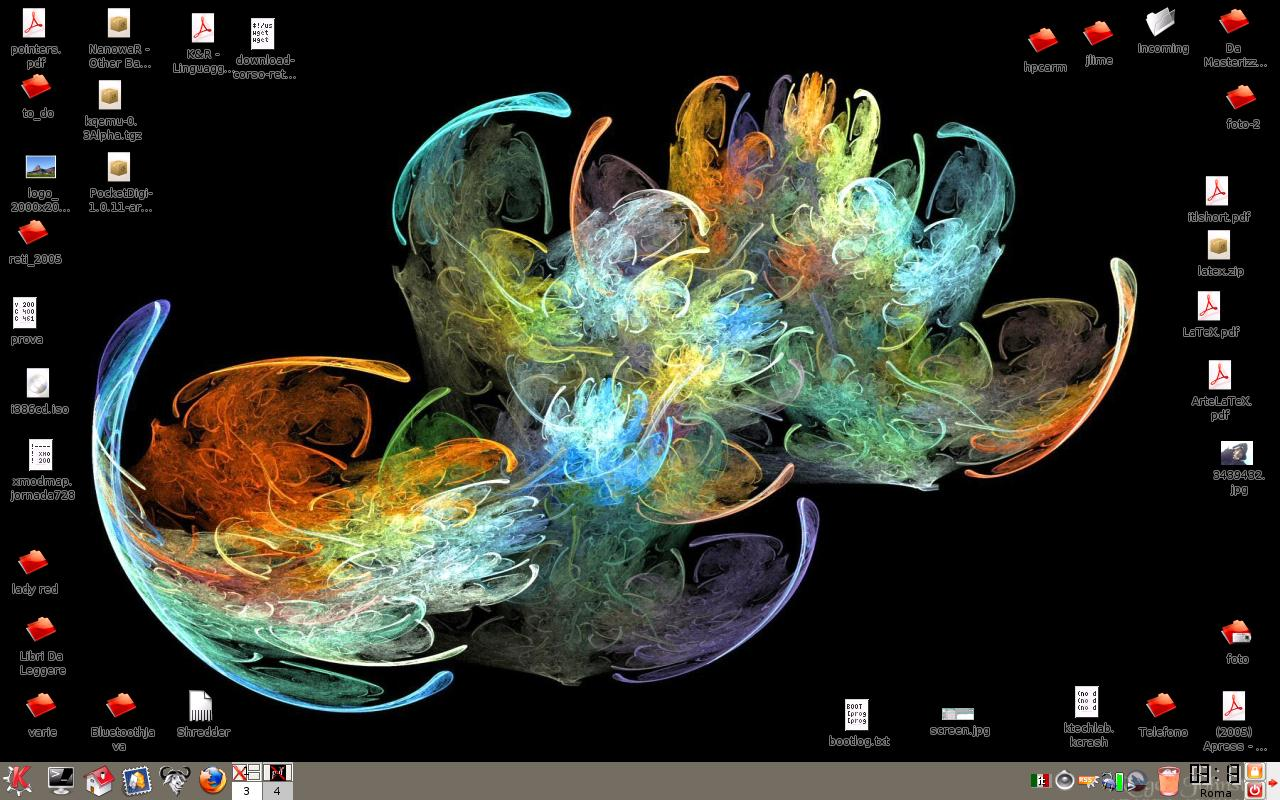
\includegraphics[width=4cm,height=3cm]{immagini/screen.eps}
}


\end{slide}



\begin{slide}{Perchè programmare con GNU/Linux?}
{\small
Perchè si dovrebbe scegliere GNU/Linux per programmare?

La risposta è semplice. 

Il progetto GNU fornisce una miriade di
applicazioni e librerie per programmare, in modo completamente gratuito.

Linux può vantare altissime prestazioni ed è capace di reggere forti
carichi di lavoro. Oltretutto, è quasi completamente immune da virus ed
in generale è spaventosamente più sicuro di Windows.

Inoltre, ci sono tonnellate di strumenti potentissimi... E liberamente
disponibili. Vediamone qualcuno.
}
\end{slide}


\begin{slide}{Il compilatore GCC}
GCC, che sta per GNU Compiler Collection, è una suite di compilatori
liberi e gratuiti per GNU/Linux. Supportano C, C++, ObjectiveC, ADA,
Fortran e Java.

Oltretutto, possono compilare per svariate piattaforme: x86, ARM, PPC,
MIPS, Alpha... Tant'è vero che GNU/Linux può essere installato quasi
dappertutto: su cellulari, palmari, pc, apple machintosh, hpc, server,
thin client, xbox, ipod, playstation2, playstation3, sega dreamcast,
gamecube, schede integrate...

\end{slide}


\begin{slide}{Sistemi di revisione}
{\small
Il progetto GNU mette a disposizione anche dei \emph{sistemi di
revisione}. Cosa sono? Un sistema di revisione è un programma che
permette a più persone di lavorare allo stesso programma insieme,
gestendo automaticamente le modifiche apportate al codice.

In questo modo, gestire progetti è più semplice.

Alcuni RCS famosi sono:
\begin{itemize}
	\item[-] CVS
	\item[-] Subversion
	\item[-] Git
\end{itemize}
}
\end{slide}


\end{document}
